% Abschlussarbeit am Ende der Oberschule
% Facharbeit zum parallelen Programmierparadigma
% Thomas Mittermair
% Oberschulzentrum J. Ph. Fallmerayer Brixen

\chapter{Einleitung und Motivation}

	\section{Einführung in die Problematik der Parallelisierung}

		Der Begriff der \textit{Parallelität} existiert nicht nur im Bereich der Informatik, sondern vor allem im Alltag und in der Natur ist selbiger oft vorzufinden und somit allgegenwärtig. Um zu begreifen, worum es sich bei Parallelität handelt, muss zunächst klargestellt werden, worin der Unterschied zwischen Sequentialität und Parallelität liegt.

		\subsection{Begriffe der Sequentialität und Parallelität}

			Die Ausdrücke \textit{Sequentialität} und \textit{Parallelität} stellen Schlüsselbegriffe im Zusammenhang mit dieser Arbeit dar. Der Online-Duden gibt für diese beiden Begriffe die nun folgenden Definitionen.
			
			\begin{description}
			  \item[Sequentialität]
				  Der Begriff \textit{Sequentialität} hängt eng mit dem Adjektiv \textit{sequenziell} zusammen. Vorgänge, die sequenziell ablaufen, spielen sich aufeinander folgend und der Reihe nach ab. \cite{SequentiellDuden}
			  \item[Parallelität]
				  Der Begriff \textit{Parallelität} hängt eng mit dem Adjektiv \textit{parallel} zusammen. Vorgänge, die parallel ablaufen, spielen sich gleichzeitig und synchron ab. \cite{ParallelDuden}
			\end{description}

			\subsubsection{Sequentialität und Parallelität im Alltag und in der Natur}
			
				Jeder Mensch ist, oft ohne davon Kenntnis zu nehmen, täglich mit sequentiellen und parallelen Vorgängen und Abläufen konfrontiert. Ein alltägliches Beispiel für Sequentialität ist der Begriff von Zeit, denn eine Sekunde vergeht erst, sobald die vorherige Sekunde vollkommen abgelaufen ist. Zeit läuft somit vollkommen sequentiell ab, wodurch das Kausalitäts-Prinzip, also das Prinzip von Ursache und Wirkung, erst möglich wird, denn hätte die Zeit diese Eigenschaft nicht, so wären Ursache und Wirkung nicht klar voneinander unterscheidbar. Folglich geschieht in der Natur nichts ohne Grund, und das bedeutet wiederum, dass es zu jedem beliebigen Ereignis ein anderes Ereignis gibt, das in der Vergangenheit liegt und das nachfolgende Ereignis hervorruft. \cite{Kausalitaet} Viele Vorgänge in der Natur laufen hingegen parallel ab. Beispielsweise findet stets eine simultane Weiterentwicklung statt, denn jeder Mensch und auch jede Pflanze entwickeln sich gleichzeitig, und nicht nacheinander, weiter. \cite{ParaProgLoogen}
				
			\subsubsection{Sequentialität und Parallelität in der Informatik}
				\label{SequUndParaInformatik}
				
				Die Informatik ist eine Wissenschaft, die in vielen Bereichen das Ziel verfolgt, Objekte und auch Abläufe der realen Welt auf Ebene von Rechnern möglichst realitätsgetreu nachzubilden. Ein informatisches Modell der Wirklichkeit soll folglich so nahe wie möglich an die zu modellierende Begebenheit herankommen. Ein in diesem Zusammenhang oft genanntes Beispiel ist das objektorientierte Programmierparadigma. Dabei werden Objekte der realen Welt durch Datenstrukturen im Computer nachgeahmt. Dies erlaubt es, Sachverhalte in der Realität nahezu direkt und ohne große Abänderungen in einer objektorientierten Programmiersprache zu modellieren. \cite{Objektorientierung} Ähnliches gilt für die Sequentialität und Parallelität in der Informatik. Um zu verstehen, wie diese beiden Gegensätze in der Informatik zusammenhängen und realisiert werden, muss zunächst erläutert werden, wie ein Prozessor Befehle abarbeitet.
				
				\begin{description}
			  		\item[Ausführungsschema eines Prozessors]
						Der Prozessor, oft auch CPU (Central Processing Unit) genannt, ist das Herzstück eines Rechners. Er ist die Komponente, welche für die Ausführung und Abarbeitung der Befehle zuständig ist. Ein Prozessor kann dabei im Normalfall, also sofern er nur aus einem Kern besteht, nur eine Operation zugleich ausführen. Diese Eigenschaft leitet sich vom Schema ab, nach welchem die Mehrheit aller im Moment auf dem Markt befindlichen CPUs arbeiten. Dabei handelt es sich um den \textit{Von-Neumann-Zyklus}, allgemeiner auch als \textit{Befehlszyklus} bekannt.
						Die Abarbeitung eines Befehls geschieht dabei meist nach dem folgenden Schema:
						
						\begin{enumerate}
							\item \textbf{Instruction-Fetch-Phase (IF), Befehlholungs-Phase}: In dieser Phase wird der Befehlscode vom Hauptspeicher in ein Register des Prozessors geladen.
							\item \textbf{Instruction-Decode-Phase (ID), Befehldekodierungs-Phase}: Der in ein Register geladene Befehl wird nun decodiert, um den Befehl weiterverarbeiten zu können. In dieser Phase wird der Befehl folglich analysiert, um Informationen zur Art des Befehls sowie zu Art und Anzahl der beteiligten Operanden und weitere Details zu ermitteln.
							\item \textbf{Fetch-Operands-Phase (FO), Operandennachladungs-Phase}: In dieser Phase werden die Operanden, welche zur Abarbeitung des Befehls notwendig sind, in die Register nachgeladen. Bei Befehlen ohne Operanden bleibt diese Phase leer, da sie in diesem Fall nicht benötigt wird. Die Fetch-Operands-Phase kann auch als Unterphase der Instruction-Decode-Phase betrachtet werden, da die Operanden, welche in der Instruction-Decode-Phase ermittelt wurden, in dieser Phase aus dem Hauptspeicher in die Register geladen werden.
							\item \textbf{Execute-Phase (EX), Befehlausfühungs-Phase}: In dieser Phase kann der Befehl nun, beispielsweise unter Verwendung des Rechenwerkes, ausgeführt werden. Hierbei wird der geladene Befehl unter Verwendung der geladenen Operanden (falls vorhanden) abgearbeitet.
							\item \textbf{Write-Back-Phase (WB), Resultat-Rückschreibungs-Phase}: In dieser Phase werden die Ergebnisse aus der Execute-Phase in den Speicher (z.B. in ein anderes Register oder auch in einen externen Speicher) zurückgeschrieben. Bei Befehlen ohne Resultat bleibt diese Phase leer, da sie nicht benötigt wird.
						\end{enumerate}
						
						Jeder einzelne Befehl durchläuft dieses Schema, das bedeutet, nachdem ein Befehl die Write-Back-Phase abgeschlossen hat, kann der nächste Befehl mit der Instruction-Fetch-Phase beginnen. \cite{PhasenBefehlsbearbeitung} \cite{FunktionsweiseComputersysteme}\\
						
						Diese Sequentialität des Befehlszykluses soll nun an Hand eines Beispiels der Abarbeitung von drei Befehlen verdeutlicht werden.
						Die Abbildung \ref{fig:BefehlszylusOhnePipelining} soll diesen Vorgang grafisch veranschaulichen.
						
						\begin{figure}
							\centering	
							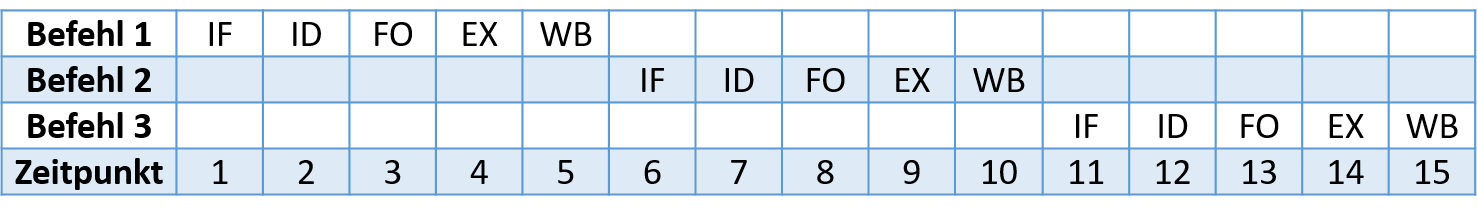
\includegraphics[width=11cm]{Abbildungen/Befehlszylus_ohne_Pipelining.png}
							\caption{Grafische Darstellung der Abarbeitung von drei Befehlen nach dem Schema des Befehlszykluses.}
							\label{fig:BefehlszylusOhnePipelining}
						\end{figure}
				\end{description}
			
				Für eine geraume Zeit in der Geschichte der Rechner war die sequentielle Abarbeitung auch die einzig Mögliche. Bei der Modellierung von Abläufen der Realität, die aus parallelen Vorgängen bestehen, führt die Sequentialisierung zu einer künstlichen Einschränkung, da parallel ablaufende Vorgänge in einem hochwertigen Modell auch parallel ablaufen müssen.
				Um eine bessere Modellierung von parallelen Vorgängen zu ermöglichen, musste folglich ein neues Programmierparadigma definiert werden, welches die Parallelität berücksichtigt. Selbiges ist heute unter dem Namen \textit{Paradigma der Parallelen Programmierung} oder auch \textit{Paralleles Programmierparadigma} bekannt und wird oft eingesetzt. Dieses Paradigma erlaubt es, Parallelverarbeitung auf Ebene der Informatik zu realisieren. Wie und mit welchen Konzepten dies geschieht bzw. geschehen kann, soll im Verlauf dieser Arbeit klar werden.
				
	\section{Gründe für das parallele Programmierparadigma}
				
		Neben der besseren Modellierung von parallelen Vorgängen bietet die Parallelisierung noch einige weitere Vorteile. Schon seit einigen Jahren wird die parallele Programmierung im Bereich des Hochleistungs-Rechnens verwendet. Genauere Simulationen oder auch die Simulationen von komplexeren Problemen benötigen immer mehr Rechenleistung und auch Speicherplatz. Ein oft genanntes Beispiel sind in diesem Zusammenhang die Wetter-Simulationen, welche auf komplizierten mathematischen Modellen basieren. Das Vorhersagen der zukünftigen Entwicklung in der Atmosphäre ist nur durch die Verwendung eines Modells und einer daraus resultierenden Simulation möglich.
		Die Schwierigkeit bei Computer-Simulationen liegt allerdings darin, dass sie meist einen großen Rechenaufwand nach sich ziehen. Ein nicht leistungsfähiger Rechner kann die Simulation selbst oder auch die Genauigkeit des resultierenden Ergebnisses erheblich einschränken. Aus diesem Grund werden Parallelrechner\footnote{Ein Parallelrechner ist ein Rechner, der über mehrere Ausführungseinheiten (z.B. Kerne oder Prozessoren) verfügt und somit echte Parallelverarbeitung unterstützt.} oft im Zusammenhang mit Computersimulationen verwendet. Um solche Rechner ausnutzen zu können, muss die durchzuführende Berechnung in mehrere, kleinere Teile zerlegt werden, welche dann den einzelnen, parallelen Abarbeitungseinheiten zugeordnet werden können. Diese einzelnen Berechnungen sollten unabhängig voneinander ablaufen, und auch der Algorithmus, der angewendet wird, muss in parallel ausführbare Einheiten zerlegbar sein. Um eine parallele Ausführung zu ermöglichen, muss der Algorithmus allerdings in einer Programmiersprache verfasst werden, welche entweder die Parallelisierung direkt durch Hinzunahme von externen Bibliotheken oder auch durch spezielle Compiler-Direktiven unterstützt, welche zu einer gewöhnlichen Programmiersprache wie beispielsweise C oder Java hinzugefügt werden. \cite{ParaProgRauber}\\
		
		\subsection{Möglichkeiten der Leistungserhöhung}
			\label{MoeglichkeitenLeistungserhoehung}
		
			Eine erhöhte Rechenleistung kann allerdings nicht nur durch Parallelisierung erreicht werden kann. Da die CPU, wie bereits erwähnt, Befehle im einfachsten Fall nur sequentiell abarbeiten kann, eröffnen sich intuitiv zwei Möglichkeiten der Leistungssteigerung:
		
			\begin{enumerate}
				\item Die erste Variante der Erhöhung der Performance besteht in der Beschleunigung der Abarbeitungszeit, die der Prozessor für einen Befehl benötigt. Dieser Lösungsansatz wirkt zunächst passend, da die Prozessoren immer kleiner und billiger werden. Doch diese Entwicklung zu immer kleineren, leistungsfähigeren CPUs ist gewissen physikalische Begrenzungen, wie beispielsweise der Lichtgeschwindigkeit als natürliche obere Grenze der Signalübertragungsgeschwindigkeit, unterworfen. Das Erreichen von Fortschritten bei der Erhöhung der Einprozessorleistung wird folglich immer schwieriger. \cite{GrundlagenParallelisierung}
				\item Angesichts des obigen Problems rücken die Fortschritte in der Netzwerktechnik in den Vordergrund. Die Verbindungen zwischen Rechnern werden immer besser, die Geschwindigkeiten höher und die Bandbreiten größer. Somit wird es in Zukunft einfacher, mehrere Prozessoren miteinander zu verbinden, sodass sie parallel an einem gemeinsamen Problem arbeiten, als die Leistung der einzelnen Komponenten zu erhöhen. \cite{GrundlagenParallelisierung} Solche sogenannte Parallelrechner sind folglich die Zukunft des Hochleistungsrechnens.
			\end{enumerate}

		\subsection{Mooresches Gesetz}
		
			Einer der Mitbegründer von Intel, Gordon Moore, formulierte im Jahr 1965 das nach ihm benannte Mooresche Gesetz. Dieses besagt, dass sich die Anzahl der Transistoren, welche in einem Prozessor enthalten sind, in etwa alle 18 Monate verdoppelt. Diese Aussage traf Moore in Bezug auf die sich damals schnell entwickelnde Halbleiter-Industrie. Zehn Jahre später, im Jahr 1975, relativierte er die von ihm formulierte Regel, indem er die Verdopplung der Anzahl der Transistoren in einem Chip von nun an auf in etwa alle zwei Jahre voraussagte.\\
			Im Jahr 2003 hielt Moore einen Vortrag über die Zukunft der Halbleiterbranche an der \textit{International Solid-State Cicuits Conference (ISSCC)}, während welchem er sich eingestand, dass das nach ihm benannte Gesetz wohl in den nächsten Jahren seine Gültigkeit verlieren würde. \cite{EndeHardwareMiniaturisierung}\\
			Schenkt man Moore und den Gesetzen der Physik Glauben, so wird die zweite der unter Kapitel \ref{MoeglichkeitenLeistungserhoehung} genannten Möglichkeit die Zukunft des Hochleistungsrechnens in der Informatik bestimmen.
			Die Abbildung \ref{fig:MoorschesGesetz} verdeutlicht nochmals den Zusammenhang zwischen der historischen Entwicklung der Anzahl der Transistoren auf einem Prozessor und dem Mooreschen Gesetz. Dabei sei erwähnt, dass die Skalierung der y-Achse dieses Diagrammes keineswegs linear ist, sondern logarithmisch erfolgt.
		
			\begin{figure}
				\centering	
				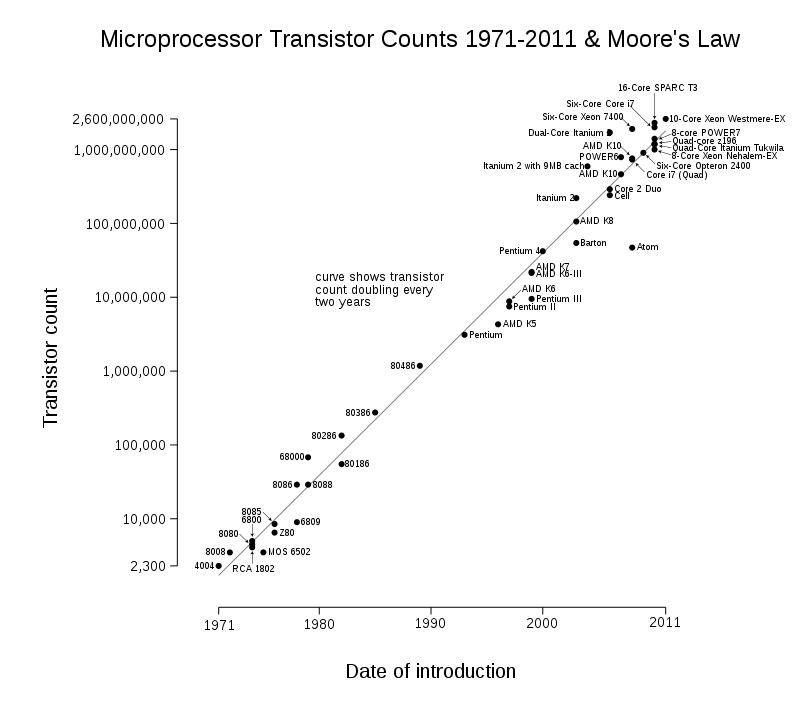
\includegraphics[width=11cm]{Abbildungen/Moorsches_Gesetz.png}
				\caption{Zusammenhang zwischen der Anzahl der Transistoren in einem Prozessor und dem Mooreschen Gesetz.}
				\label{fig:MoorschesGesetz}
			\end{figure}
		
		\subsection{Trends im Hochleistungsrechnen}
		
			Auch im Bereich des Hochleistungsrechnens werden zunehmend immer mehr Prozessoren verbunden, anstatt wenige leistungsstarke CPUs zu verwenden. Die großen Rechenzentren, wie beispielsweise das Leibniz-Rechenzentrum der Bayrischen Akademie der Wissenschaften (LRZ), verwenden sogenannte Super-Computer, welche aus tausenden von Prozessoren bestehen. Das LRZ ist beispielsweise im Besitz eines Rechners mit dem Namen \textit{SuperMUC}, welcher sich in der Nähe der deutschen Großstadt München befindet. Dieser besteht aus mehr als 241.000 Prozessor-Kernen und erreicht eine Spitzenleistung von mehr als 6,8 Petaflop/s, also mehr als $6,8\cdot10^{15}$ Floating Point Operations Per Second (Gleitkommazahl-Operationen pro Sekunde). Damit ist selbiger einer der aktuell schnellsten Super-Computer. \cite{LRZ}\\
			Somit wird klar, dass das parallele Programmierparadigma in Zukunft wohl noch an Bedeutung gewinnen wird und sich eine Auseinandersetzung mit diesem mittlerweile breitgefächerten Gebiet der Informatik lohnt.